% !TeX root = ../../main.tex

\chapter{Konzept}
In diesem Abschnitt wird kurz unser Konzept für die Umsetzung von Sfm erläutert. 
Insbesondere wird dabei erläutert, was in den einzelnen Schritten durchgeführt wird, und warum diese Schritte notwendig sind.
Details zur Implementierung werden in Kapitel~\ref{sec:implementation} beschrieben.
Das Konzept ist eine Kommandozeilen-Applikation, welche eine Pipeline mit Prozessen zur Rekonstruktion von Bildpunkten bereitstellt.
Die Pipeline ist in Abb.~\ref{fig:concept-pipeline} dargestellt.
Parameter, die für die einzelnen Prozesse benötigt werden, werden als Kommandozeilen-Argumente übergeben.

Der erste Prozess \emph{Kalibrierung} bestimmt die Parameter der Kamera, mit der die Bilder zur Rekonstruktion aufgenommen wurden.
Dieser Schritt ist nötig, da bei der Rekonstruktion die Kalibrierungsmatrix K benötigt wird.
Diese Matrix enthält Informationen über die Brennweite der Kamera und der Position des Hauptpunkts im Bild.
Des Weiteren wird bei der Kalibrierung auch die Verzerrungsparameter der Kameralinse bestimmt.
Damit kann die Verzerrung in den Bildern reduziert werden, was zu genaueren Ergebnissen beim Rekonstruieren führt.
Die Kalibrierung wird mit Hilfe eines Kalibrierungsobjekts durchgeführt.
Es wurde sich bewusst gegen die Auto-Kalibrierung entschieden, da dies nicht immer möglich ist sie anzuwenden~\cite{remondino_2005}.
Dementsprechend müssen zusätzliche Bilder für die Kalibrierung vom Nutzer bereitgestellt werden.
Der Nutzer muss dabei nur einen Ordnerpfad angeben, in dem sich die Bilder für die Kalibrierung befinden.
Das Kalibrieren der Kamera kann sehr zeitaufwendig sein.
Daher wird die Möglichkeit bereitgestellt, die Kameraparameter in einer Datei zu exportieren.
Diese Datei kann dann geladen werden, so dass eine weitere Kalibrierung mit dem Schachbrettmuster nicht mehr nötig ist. 
Es werden jedoch keine weiteren Features für die Verwaltung der Kalibrierungen angeboten.
Der Nutzer ist also selbst dafür verantwortlich zu wissen, welche Datei zu welcher Kamera gehört und welche Kalibrierungsdatei für die Pipeline benötigt wird. 

Der zweite Prozess umfasst das Feature Matching, welches benötigt wird, um korrespondierende Punkte in verschiedenen Bildern von einem Objekt zu finden.
Diese Bilder werden wie bei der Kalibrierung vom Nutzer bereitgestellt, in dem ein Ordnerpfad angeben wird, der alle Bilder enthält. 
Die Bilder werden in alphabetischer Reihenfolge geladen und nach Keypoints und ihren Deskriptoren durchsucht.
Anschließend werden Paare aus benachbarten Bildern gebildet, in denen nach übereinstimmenden Keypoints gesucht werden.
Somit ist es Aufgabe des Nutzer, die Bilder so zu sortieren, so dass es möglichst wenig Bewegung zwischen aufeinanderfolgenden Bildern gibt und mehr Übereinstimmungen gefunden werden können.
Die korrespondierenden Bildpunkte, welche sich aus den Keypoints ergeben, werden im nächsten Prozess zum Rekonstruieren der Bilder genutzt.  

Im dritten Prozess \emph{Rekonstruktion} wird die Geometrie der Szenen der Bildpaaren ermittelt und Raumpunkte durch die korrespondierende Bildpunkte bestimmt.
Dabei werden die Positionen der Kameras der vorherigen Bildpaare beachtet, damit die Weltpunkte eines Bildpaares im selben Koordinatensystem ausgedrückt werden.
Des Weiteren wird mit Hilfe der bereits bestimmten Weltpunkten die Skalierung einer Szene bestimmt.
Dadurch passen die Weltpunkte der einzelnen Szenen später beim Zusammenführen besser zusammen.
Die Schritte, die bei der Rekonstruktion durchgeführt werden, und ihre Mathematik werden in XXX erklärt.

Der vierte und letzte Prozess der Pipeline \emph{Export} sammelt die rekonstruierten Weltpunkte und bestimmt ihre Farben aus den Bildern.
Die Punkte und ihre Farbinformationen werden anschließend in einem einfachen Format als Datei gespeichert.
Diese Datei kann dann mit Programmen wie Blender oder Meshlab geladen, betrachtet und editiert werden.
Dieser Prozess und das Dateiformat werden in XXX beschrieben.


\begin{figure}
    \centering
    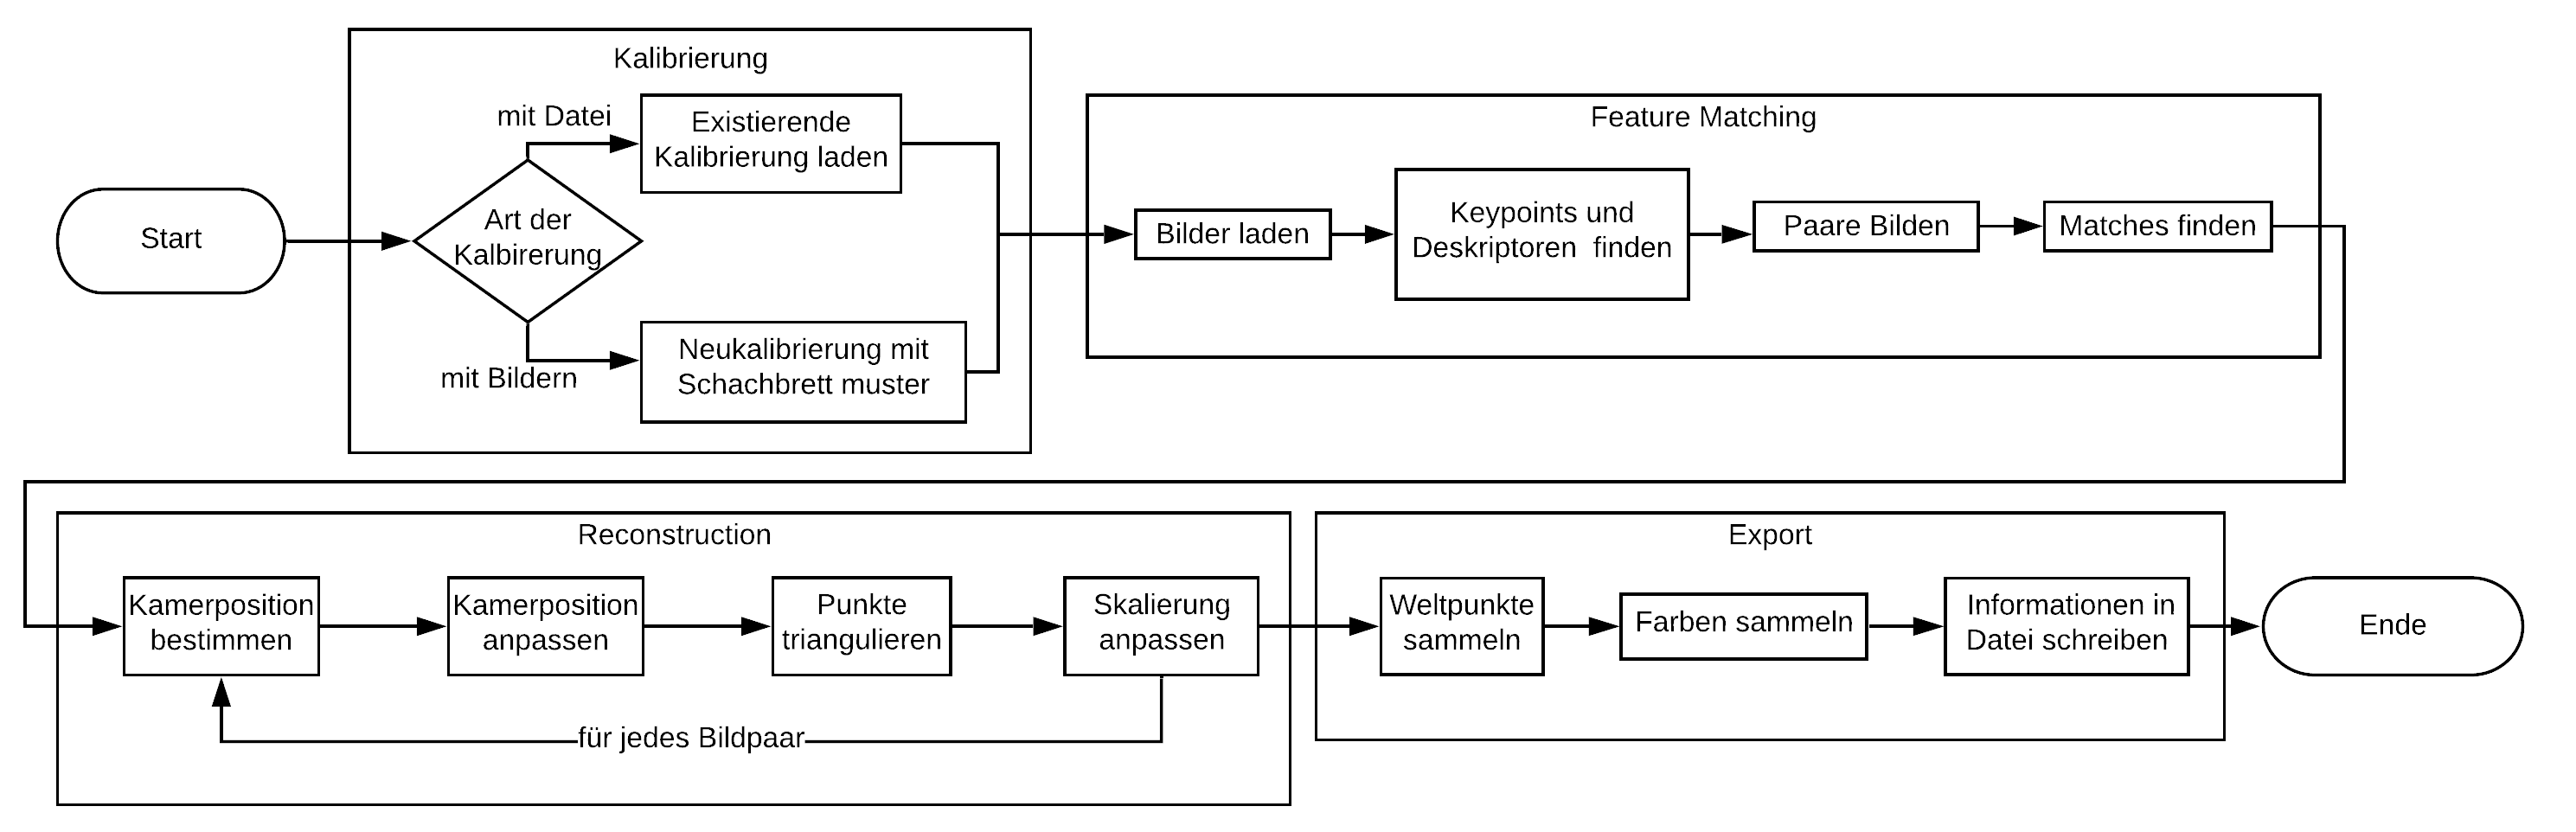
\includegraphics[width=\textwidth]{src/img/konzept-pipeline.png}
    \caption{Rekonstruktierungspipline des Konzepts}
    \label{fig:concept-pipeline}
\end{figure}
